% IEEE two-column source for the Assessment Task 3 group manuscript.
% Measured numbers are copied from cloud/benchmark/ and tools/batch_results.csv.
% Author and group identifiers remain placeholders by instructor submission convention.
\documentclass[conference]{IEEEtran}

\usepackage{cite}
\usepackage{amsmath,amssymb,amsfonts}
\usepackage{graphicx}
\usepackage{textcomp}
\usepackage{xcolor}
\usepackage{booktabs}
\usepackage{array}
\usepackage{url}

\title{Post-Flood Water-Quality Monitoring at the Edge:\\
Store-and-Forward Telemetry, Hysteresis Alarms, and Cloud Triage}

\author{
\IEEEauthorblockN{[Group member 1], [Group member 2], [Group member 3], Sambid Shrestha}
\IEEEauthorblockA{ITS67404 Internet of Things -- Assessment Task 3 \\
{[}Institution{]}, {[}City{]}, {[}Country{]} \\
{[}email addresses{]}}
}

\begin{document}

\maketitle

\begin{abstract}
Post-flood water safety depends on detecting contamination early while tolerating the
network interruptions that typically follow a flood. This paper presents an end-to-end
monitoring chain built from virtual sensing nodes, an SQLite store-and-forward buffer,
MQTT over TLS, and a ThingsBoard cloud deployment. Edge signal processing combines
validity gates, a Hampel filter, a Brown water-quality index, and a hysteresis alarm
engine with explicit deadbands and consecutive-sample debounce. The cloud side exports
a device profile with nine native alarm rules, three devices, an eight-widget triage
dashboard, and a server-side water-quality rule chain. A scripted demonstration
exercises baseline, silt intrusion, supply interruption, network outage, recovery, and
fault injection. The evaluation reports end-to-end latency, message delivery ratio,
alarm activation delay, buffer-flush throughput, recovery time, and data loss. In the
measured deployment, 528 of 530 live rows reached the tenant with a mean latency of
1.46~s; across the outage run the delivery ratio was 99.86\,\%, 96 buffered rows
replayed at 1.55~rows/s, and recovery took 61.94~s with one row lost. The results
establish the operating envelope of the prototype and expose operational limits that
must be addressed before production use.
\end{abstract}

\begin{IEEEkeywords}
Internet of Things, water quality, MQTT, TLS, store-and-forward, ThingsBoard, hysteresis, alarms
\end{IEEEkeywords}

\section{Introduction}
\label{sec:intro}

Post-flood water supplies can remain in use after turbidity and microbial indicators
have risen above safe limits. Continuous sensing is therefore useful only when the
measurement chain survives intermittent connectivity and reports excursions without
generating repeated, contradictory alarms. This work addresses both requirements with a
low-cost virtual-node implementation and a cloud configuration that can be exported and
reproduced. The contribution of this work is fourfold. First, a deterministic virtual
sensor model generates coupled pH, turbidity, TDS, temperature and flow samples for
three nodes, including onset offsets that emulate an advancing contamination plume.
Second, the edge pipeline combines physical validity gates, a Hampel filter,
temperature compensation, a Brown water-quality index and a hysteresis alarm engine
whose deadbands and consecutive-sample debounce are evaluated on every sample. Third,
a durable SQLite queue with explicit pending/inflight/synced states and
PUBACK-confirmed MQTT/TLS publishing preserves acquisition timestamps across
connectivity loss. Fourth, the tenant configuration is supplied as importable
artifacts---device profile, three devices, an eight-widget dashboard, nine alarm
rules and a server-side WQI chain---together with a benchmark tool that obtains the
six quantitative metrics required by the assessment from the deployed platform.

The remainder of the paper describes the architecture and edge processing
(Sections~II--IV), the cloud implementation and tool selection (Sections~V--VII), the
measured results and operational lessons (Section~VIII), and the conclusions and
future work (Sections~IX--X). Appendices~A--B document the telemetry contract and
the reproduction procedure.

\section{System Architecture}
\label{sec:architecture}

The prototype is organised as five stages, as shown in Fig.~\ref{fig:architecture}.
Three virtual nodes (\texttt{node-a}, \texttt{node-b}, \texttt{node-c}) generate
timestamped readings for pH, turbidity, total dissolved solids (TDS), water
temperature and flow. A scenario controller advances through baseline, silt
intrusion, supply interruption and recovery phases with a 12$\times$ acceleration
factor, so a production event lasting tens of minutes is compressed into a
demo-scale interval. Each raw sample passes through validity gates, a Hampel
filter and temperature compensation before the Brown water-quality index (WQI)
and alarm state are computed. The resulting payload is persisted locally before
any network operation.

\begin{figure}[t]
\centering
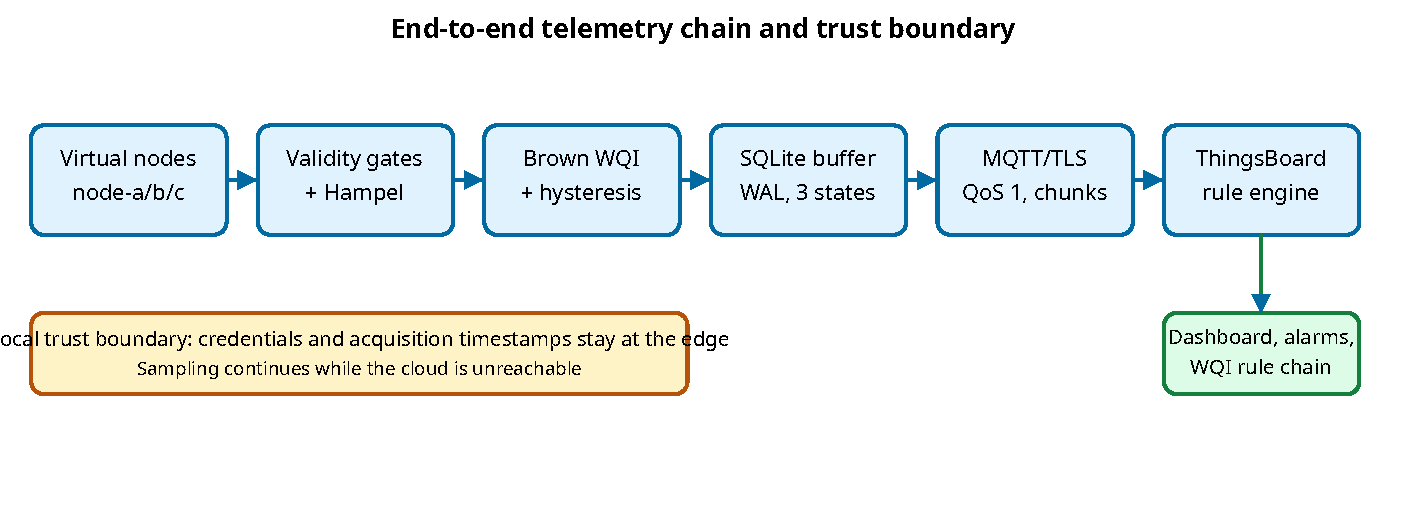
\includegraphics[width=\columnwidth]{figures/architecture.pdf}
\caption{End-to-end data flow and trust boundary of the prototype.}
\label{fig:architecture}
\end{figure}

The durable queue is drained by one publisher per node. Each publisher uses its
own ThingsBoard access token and a stable MQTT client id over TLS on port 8883.
Only the rule engine, dashboard and alarm service reside in the tenant; the
access tokens and tenant credentials remain in a local, gitignored environment
file and are never embedded in exported artefacts. This is the trust boundary
of the deployment: the edge may continue sampling and buffering when the cloud
is unreachable, but a cloud compromise cannot rewrite the local acquisition
timestamps.

\subsection{Deployment Model and Scenario Control}

Each virtual node is configured with an identifier, a geographic coordinate, a
deterministic random seed, an intrusion amplitude and an onset offset. The three
amplitudes are 500, 825 and 1250~NTU and the onset offsets are 0, 20 and 40~s, so
a forced silt intrusion reaches the nodes in sequence rather than
simultaneously; this makes cross-node correlation meaningful. The scenario clock
is accelerated by a factor of twelve relative to wall time. An operator can force
phases from the CLI: baseline, silt intrusion, supply interruption and recovery,
together with outage toggling, node power off/on, stuck-sensor injection,
authentication retry, pause and quit. The demonstrated live run used a one-second
tick, a batch size of 50 rows and a 6048-row bounded queue; the default
configuration uses a five-second tick. A powered-off node continues to emit
inactivity status built from its last processed values without polluting its
Hampel windows with synthetic samples.

\begin{table}[t]
\caption{Operator commands used in the scripted demonstration}
\label{tab:commands}
\centering
\scriptsize
\begin{tabular}{@{}ll@{}}
\toprule
Key & Action \\
\midrule
\texttt{b/s/i/r} & force baseline, intrusion, interruption, recovery \\
\texttt{o} & toggle connectivity outage \\
\texttt{k/K} & power node-a off/on \\
\texttt{f/F} & inject/clear stuck-sensor fault on node-a \\
\texttt{a} & retry authentication after token correction \\
\texttt{p/q/h} & pause, quit, or print help \\
\bottomrule
\end{tabular}
\end{table}

\subsection{Failure Model and Design Requirements}
\label{sec:failure-model}

The deployment targets six failure modes observed or anticipated during the
demonstration. Table~\ref{tab:failures} maps each mode to the mechanism that
contains it and to the evidence used to check the mechanism. The design goal is
not to eliminate every failure but to preserve the audit trail and to make each
failure visible in a saved log or a tenant export. In particular, a cloud
outage must not stop local sampling, an oversized MQTT packet must not discard a
batch, and a sensor fault must not silently replace a valid historical value.

\begin{table}[t]
\caption{Failure modes, mitigations, and evidence}
\label{tab:failures}
\centering
\scriptsize
\begin{tabular}{@{}lll@{}}
\toprule
Failure & Mitigation & Evidence \\
\midrule
Cloud unreachable & SQLite + paused flush & OUTAGE/BUFFER log \\
Oversize packet & 1800-byte chunks & PUBACK per chunk \\
Session takeover & stable node client id & three publishers \\
Sensor fault & gates + last-valid value & VALIDITY/FAULT log \\
API drift & \texttt{agg=NONE}, per-device alarms & benchmark reports \\
Token expiry & env-only short-lived JWT & refreshed for run 2 \\
\bottomrule
\end{tabular}
\end{table}

The quantitative acceptance conditions are likewise tied to evidence: latency
requires at least 200 messages carrying \texttt{server\_received\_ms}, alarm delay
requires at least ten paired alarm events, and delivery ratio, throughput,
recovery and loss require a run that contains a completed outage. Section~VIII
reports the measured sample sizes beside each value so that these conditions can
be checked without re-running the experiment.

\section{Edge Signal Processing}
\label{sec:edge-dsp}

Physical validity gates reject samples outside plausible ranges (pH 0--14,
turbidity 0--4000~NTU, TDS 0--5000~ppm, temperature $-5$--60~$^\circ$C and
flow 0--500~L/min). Endpoint readings such as pH~0 or pH~14 are classified as
OPEN/SHORT, non-finite or out-of-range values as SATURATION, and implausible
pH/TDS combinations as SANITY failures. A channel that remains byte-identical
for nine consecutive samples is flagged STUCK. In every case the gate
substitutes the most recent valid value before DSP; the raw value and flag are
retained for audit.

\begin{table}[t]
\caption{Physical validity gates}
\label{tab:validity}
\centering
\scriptsize
\begin{tabular}{@{}ll@{}}
\toprule
Flag & Condition \\
\midrule
OPEN\_SHORT & pH at 0 or 14; turbidity at 4000; temp at endpoints \\
SATURATION & non-finite or outside physical range \\
SANITY & pH $<5$ with TDS $>1000$, or pH $>10$ with TDS $<20$ \\
STUCK & byte-identical for nine consecutive samples \\
\bottomrule
\end{tabular}
\end{table}

Isolated spikes are removed by a nine-sample Hampel filter with $k=3$. The
scale estimate is $1.4826\,\mathrm{median}|x_i-\mathrm{median}(X)|$, with the
population standard deviation used as a fallback when the median absolute
deviation is zero, so a single spike in an otherwise constant run is still
detected. The filter retains the raw series in its window so a genuine step
change survives after the window fills.

The pH electrode is compensated with the Nernst slope
\begin{equation}
s(T)=\frac{2.303RT}{F}\cdot 1000 \quad [\mathrm{mV/pH}],
\end{equation}
giving $s(25\,^\circ\mathrm{C})\approx59.16$~mV/pH. Both $pH_T$ and the
25~$^\circ$C-equivalent $pH_{25}$ are published. TDS is compensated to 25~$^\circ$C
with a temperature coefficient $\alpha=0.02\,^\circ\mathrm{C}^{-1}$.

The WQI follows the no-chlorine Brown fallback from Task~2 \cite{Task2}. With
standards $S=(8.5,5.0,1000.0)$, ideals $V_0=(7.0,0.0,0.0)$ and weights
$w=(0.3692,0.6277,0.0031)$, each sub-index is
$q_i=100\max(0,(x_i-V_{0,i})/(S_i-V_{0,i}))$ and
$\mathrm{WQI}=\sum_i w_i q_i$. Bands are $\le25$ Excellent, $\le50$ Good,
$\le75$ Poor, $\le100$ Very poor and $>100$ Unsuitable.

The alarm engine applies per-rule deadbands and consecutive-sample debounce.
A value inside a deadband holds the current latch state and does not advance the
clear counter; only consecutive qualifying samples count. The payload exposes
\texttt{severity}, \texttt{active\_alarms} and \texttt{node\_inactive} so the
cloud dashboard follows edge decisions.

\subsection{Processing Pipeline and Constants}

Algorithm~1 gives the per-sample order of operations. The important property is
that persistence happens after all derived values and alarm state have been
attached but before any network operation, so a broker failure cannot lose the
audit record.

The Hampel scale estimate is computed over a nine-sample raw window. With
$m=\mathrm{median}(X)$ and $\hat{\sigma}=1.4826\,\mathrm{median}|x_i-m|$, a sample is
replaced by $m$ when $|x_i-m|>3\hat{\sigma}$; if $\hat{\sigma}=0$, the population
standard deviation of the same window is used so that a lone spike in a constant
run is still detected. Temperature compensation uses the Nernst slope
$s(T)=2.303RT/F$ and the ambient-to-25~$^\circ$C TDS correction

\begin{equation}
\mathrm{TDS}_{25}=\frac{\mathrm{TDS}_{T}}{1+\alpha(T-25)},\qquad \alpha=0.02\,^\circ\mathrm{C}^{-1}.
\end{equation}

Each Brown sub-index is $q_i=100\max\{0,(x_i-V_{0,i})/(S_i-V_{0,i})\}$, and
$\mathrm{WQI}=\sum_i w_iq_i$ with the weights listed in Table~\ref{tab:constants}.
The latch update is a three-state counter: while inactive, $b$ consecutive
breaches raise the latch; while active, $c$ consecutive clear-eligible samples
lower it; a deadband sample leaves the latch unchanged but resets $c$ to zero.
This is the formal statement of the anti-flapping behaviour used by all nine
rules, with $(b,c)=(1,1)$ for turbidity rules and $(3,3)$ for the pH and TDS
rules.

{\scriptsize
\begin{verbatim}
Algorithm 1  Per-sample edge processing (one node, one tick)
 1: raw <- sensor.sample(phase, elapsed_s)
 2: flags <- validity_gates(raw)
 3: clean <- substitute_last_valid(raw, flags)
 4: for each channel: clean[c] <- Hampel9.update(clean[c])
 5: ph_25 <- compensate_ph(ph, temp)
 6: tds <- compensate_tds(tds, temp)
 7: wqi, band <- brown_wqi(ph_25, turbidity, tds)
 8: severity, alarms <- hysteresis.evaluate(clean, now)
 9: attach severity, alarms, buffer_depth,
10:        node_inactive, validity_flags, fault
11: buffer.enqueue(ts, values)  # before publish
\end{verbatim}
}

Table~\ref{tab:constants} collects the constants used by the implementation. The
alarm windows are deliberately accelerated demonstration values; the production
intervals are listed for comparison in Section~X.

\begin{table}[t]
\caption{Edge processing constants}
\label{tab:constants}
\centering
\scriptsize
\begin{tabular}{@{}llr@{}}
\toprule
Component & Constant & Value \\
\midrule
Validity & pH / turbidity / TDS & 0--14 / 0--4000 / 0--5000 \\
Validity & temp. / flow & $-5$--60~$^\circ$C / 0--500~L/min \\
Validity & stuck lookback & 9 samples \\
Hampel & window / $k$ / MAD scale & 9 / 3 / 1.4826 \\
Compensation & Nernst slope at 25~$^\circ$C & 59.1600~mV/pH \\
Compensation & TDS $\alpha$ & 0.0200~$^\circ$C$^{-1}$ \\
WQI & standards $S$ & 8.5000, 5.0000, 1000.0000 \\
WQI & ideals $V_0$ & 7.0000, 0.0000, 0.0000 \\
WQI & weights $w$ & 0.3692, 0.6277, 0.0031 \\
Alarm & turbidity raise/clear & $>50$ / $<40$~NTU \\
Alarm & gross raise/clear & $>200$ / $<150$~NTU \\
Alarm & pH raise/clear & out 6.5000--8.5000 / in 6.7000--8.3000 \\
Alarm & TDS raise/clear & $>500$ / $<450$~ppm \\
Alarm & flow / inactivity & 30~s / 90~s \\
Transport & PUBACK timeout & 10~s \\
Transport & backoff bounds & 1--60~s \\
Transport & max MQTT payload & 1800~bytes \\
\bottomrule
\end{tabular}
\end{table}

\section{Store-and-Forward Transport}
\label{sec:transport}

The SQLite buffer uses WAL journalling and three row states: \texttt{pending},
\texttt{inflight} and \texttt{synced}. A row is inserted before the publish
attempt, claimed oldest-first and marked inflight, then marked synced only after
the broker acknowledges QoS~1 delivery. A failed publish returns the row to
\texttt{pending} with exponential backoff; an authentication refusal suspends
only that node's retries while the remaining nodes continue to drain. The queue
is bounded, and eviction prefers the oldest pending rows so a long outage cannot
grow the database without limit.

During a simulated outage the sampling threads keep writing new rows while the
flush thread pauses. On restoration, claimed batches are logged with a
\texttt{REPLAY} marker and published with their original epoch-millisecond
timestamps, so the cloud chart shows a filled chronological gap rather than a
spike at recovery time. A fair per-node claim limit prevents one backlogged
node from monopolising the global batch.

Two deployment details were required by the target tenant. First, telemetry
packets larger than approximately 2~KiB are rejected with an MQTT disconnect;
the publisher therefore splits each logical batch into JSON arrays of at most
1800 bytes and requires a PUBACK for every chunk before acknowledging the
batch. Second, each node connects with a distinct client id to avoid session
takeover when three publishers are active in the same tenant.

\subsection{Buffer State Machine and Retry Behaviour}

Table~\ref{tab:states} defines the three row states. State transitions are
guarded by a re-entrant lock and committed through SQLite WAL journalling, so a
process restart leaves inflight rows recoverable by resetting them to pending.

\begin{table}[t]
\caption{SQLite buffer row states}
\label{tab:states}
\centering
\scriptsize
\begin{tabular}{@{}lll@{}}
\toprule
State & Meaning & Transition out \\
\midrule
\texttt{pending} & generated, awaiting publish & claimed oldest-first \\
\texttt{inflight} & claimed, PUBACK outstanding & synced on ACK; pending on failure \\
\texttt{synced} & acknowledged and retained & immutable \\
\bottomrule
\end{tabular}
\end{table}

Algorithm~2 summarises the flush loop. Claiming uses a window function to cap the
number of rows taken from each node, which prevents a single backlogged publisher
from monopolising the global batch. Rows are published in timestamp order and a
failure returns the whole batch to pending with a doubled backoff, bounded by
60~s. An authentication refusal is treated differently: only the affected
node's publisher is suspended until the operator corrects its token, while the
other nodes continue to drain.

{\scriptsize
\begin{verbatim}
Algorithm 2  Durable flush and replay
 1: if outage_active: return
 2: suspended <- publishers with auth retries suspended
 3: for (node, rows) in claim(exclude=suspended,
 4:                            per_node=batch_size/nodes):
 5:     log REPLAY if batch follows an outage
 6:     chunks <- JSON arrays <= 1800 bytes
 7:     publish QoS 1 chunks, wait 10 s for PUBACK
 8:     if all acknowledged: store.ack(rows)
 9:     else: store.fail(rows); backoff <- min(60,2*b)
10: if restored and depth == 0: log BUFFER: total=0
\end{verbatim}
}

\section{Related Work}
\label{sec:related}

A minimal alternative is a raw MQTT broker with a custom web dashboard. That
approach offers transport-level flexibility but requires bespoke device
identity, credential rotation, alarm state machines, history retention and
visualisation code. ThingsBoard \cite{TB} supplies these as platform services:
per-device tokens, a rule engine with native alarm definitions, time-series
storage and exportable dashboards. The \texttt{paho-mqtt} client \cite{Paho} is
used only for the edge-to-broker link, keeping the transport swappable behind a
publisher interface for dry runs and tests.

Platform-native device management is not free of operational issues. On the
tenant used here, the legacy device-profile alarm list was hidden after import,
so the same nine rules were also supplied as individual importable alarm
documents; dashboard aliases were silently rejected, requiring direct device
identifiers; and the severity map had to derive colour from raw telemetry
because the tenant did not store the edge-published \texttt{severity} key. The
gap addressed by this prototype is therefore not another broker, but a
reproducible configuration and evidence set that survives those platform
differences while retaining an independently verified edge state machine.

Three integration patterns were considered. A broker-centric design treats
ThingsBoard as one subscriber among many; it maximises transport control but
pushes device identity, alarm latching and history retention into application
code. A flow-centric design puts correlation logic in a visual editor; this
is convenient for demonstrating simultaneous breaches, but the flow itself is
not a device registry and does not export dashboards as stable artifacts. A
platform-centric design, used here, delegates those services to the tenant and
keeps only signal conditioning and durable buffering at the edge. The trade-off
is that tenant implementation details become part of the deployment
contract: the publisher must respect the accepted packet size, the benchmark
must use the endpoints available on the current release, and the dashboard
must bind to identifiers that the tenant actually resolves. The committed
JSON files make those details reviewable instead of leaving them as
unrecorded UI actions.

\section{Implementation}

\subsection{Cloud Provisioning and Triage Dashboard}
\label{sec:cloud-ux}

The edge publishes three timestamped MQTT/TLS streams to ThingsBoard \cite{TB} over QoS 1
on the topic \texttt{v1/devices/me/telemetry}, using the Python \texttt{paho-mqtt}
client \cite{Paho}. Devices \texttt{node-a}, \texttt{node-b}, and \texttt{node-c} are
registered at 27.7172/85.3240, 27.6790/85.3190, and 27.7500/85.3700, respectively. Each
device holds its own access token, so every stream has an independent rule-engine
originator. The server-side availability timeout is 180~min in normal operation and
45~min in burst mode; this value is deliberately reported separately from the edge's
90~s \texttt{Node Inactive} alarm, which is an accelerated demonstration setting.

The committed eight-widget dashboard is derived from a six-chart ThingsBoard export that
was confirmed to render data on the target tenant. It preserves raw \texttt{NONE}
aggregation, a 24-hour timewindow, and visible sample points. The eight widgets are a pH
radial gauge, a turbidity radial gauge, a digital TDS gauge, a multi-parameter time
series, a temperature/flow chart, an OpenStreetMap severity map, a native alarms table,
and a node-status entity table. The charts and the three map markers bind directly to
the verified device identifiers; the gauges are fixed to node-a, while the alarms and
fleet tables use an explicit list of the same identifiers.

\begin{table}[t]
\caption{Eight-widget triage dashboard}
\label{tab:widgets}
\centering
\scriptsize
\begin{tabular}{@{}ll@{}}
\toprule
Widget & Primary binding \\
\midrule
pH radial gauge & \texttt{ph}, node-a \\
Turbidity radial gauge & \texttt{turbidity\_ntu}, node-a \\
TDS digital gauge & \texttt{tds\_ppm}, node-a \\
Multi-parameter series & three device IDs \\
Temperature/flow chart & three device IDs \\
OpenStreetMap severity map & three direct-device markers \\
Native alarms table & explicit device-ID list \\
Node-status entity table & explicit device-ID list \\
\bottomrule
\end{tabular}
\end{table}

After import, all eight widget shells rendered on the tenant but the first map
configuration drew no markers. Inspection showed that latest telemetry contained
\texttt{latitude} and \texttt{longitude} but not the edge-published \texttt{severity}
key. The map was rebuilt with three direct-device markers whose colour is taken from
\texttt{severity} when present and otherwise derived from \texttt{active\_alarms},
\texttt{turbidity\_ntu}, \texttt{ph}, \texttt{tds\_ppm}, and \texttt{flow\_lpm}. Red
represents Fault or Critical, orange Major, yellow Warning, and green Normal. Radio-signal
strength is not available because the virtual nodes emit no radio telemetry; it is
therefore reported as N/A rather than fabricated. The profile-to-device assignment
was verified on the tenant and is reproduced in Fig.~\ref{fig:profile}.

Availability is evaluated at two independent layers, and the paper keeps the
two numbers separate. ThingsBoard marks a device inactive after 180~min in
normal operation and 45~min in burst mode; that is a server-side connection
timeout. The edge raises \texttt{Node Inactive} after 90~s without a generated
reading, which is an accelerated demonstration value. Table~\ref{tab:availability}
summarises the distinction. Because the two timers observe different clocks and
different failure modes, agreement between them is not expected during a short
demo.

\begin{table}[t]
\caption{Availability timers at the two layers}
\label{tab:availability}
\centering
\scriptsize
\begin{tabular}{@{}lll@{}}
\toprule
Layer & Trigger & Purpose \\
\midrule
Tenant device state & 180~min / 45~min & connection liveness \\
Edge alarm engine & 90~s without samples & local node liveness \\
Flow interruption & 30~s of zero flow & supply failure \\
\bottomrule
\end{tabular}
\end{table}

\begin{figure}[t]
\centering
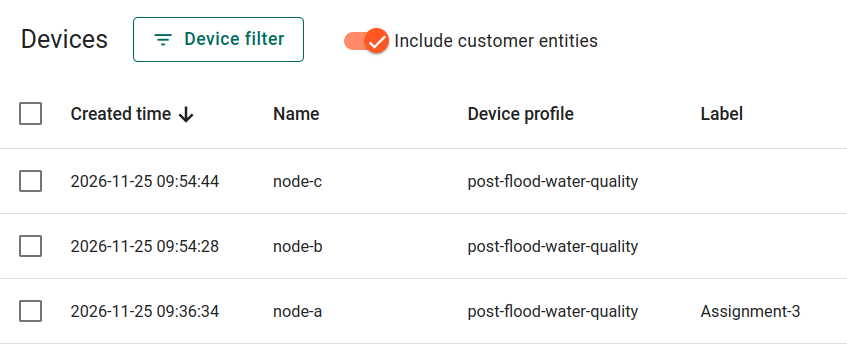
\includegraphics[width=\columnwidth]{figures/device_profile_assignment.png}
\caption{Tenant device-profile assignment for the three water-quality nodes.}
\label{fig:profile}
\end{figure}

\begin{figure}[t]
\centering
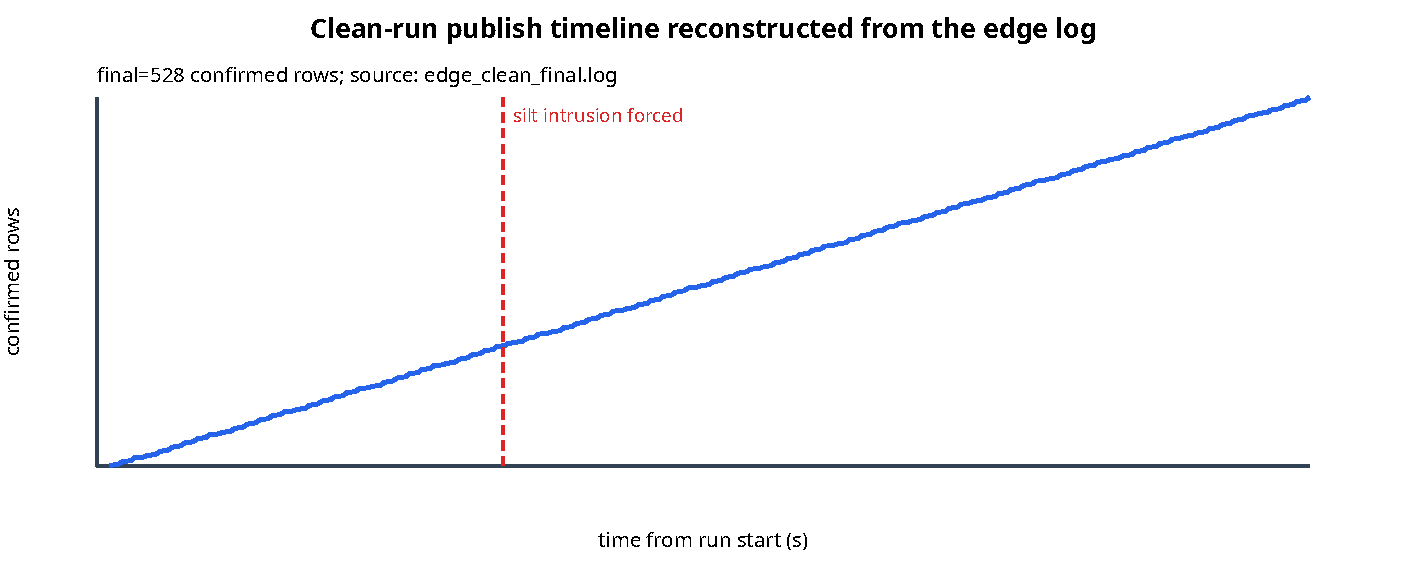
\includegraphics[width=\columnwidth]{figures/event_timeline.pdf}
\caption{Cumulative confirmed rows and the forced phase transition, reconstructed
from \texttt{evidence/edge\_clean\_final.log}; this is a log-derived timeline, not a
dash\-board screenshot.}
\label{fig:baseline}
\end{figure}

\subsection{Alarm Rules and Hysteresis Anti-Flapping}
\label{sec:alarms}

The assessment brief \cite{Brief} requires six threshold alarms, and the work division
\cite{Division} assigns their configuration to the cloud track. The alarm contract is
shipped in two deployment forms: a human-readable specification and nine importable
\texttt{ALARM} calculated-field documents, one per rule. The device profile export also
retains the older \texttt{profileData.alarms} representation for v3.x compatibility.
Current Cloud tenants may hide that deprecated list after a successful profile import,
so the per-rule files are imported through Alarm rules $\rightarrow$ Import and assigned
to the \texttt{post-flood-water-quality} profile. Together they define the six mandatory direct
rules and three mirrors of edge-derived conditions. Table~\ref{tab:rules} lists the
mandatory rules. All nine are declarative ThingsBoard rules; no custom alarm rule chain
is used for alarming.

\begin{table}[t]
\caption{Mandatory alarm rules and hysteresis deadbands}
\label{tab:rules}
\centering
\scriptsize
\begin{tabular}{@{}llll@{}}
\toprule
Alarm & Severity & Raise & Clear \\
\midrule
High Turbidity & Warning & turbidity $>50$ & turbidity $<40$ \\
Gross Contamination & Critical & turbidity $>200$ & turbidity $<150$ \\
pH Out of Range & Critical & pH $<6.5$ or $>8.5$ & $6.7\le$pH$\le8.3$ \\
High TDS & Critical & TDS $>500$ & TDS $<450$ \\
Supply Interruption & Major & flow $=0$ for 30~s & flow $>0$ \\
Node Inactive & Critical & no data for 90~s & telemetry resumes \\
\bottomrule
\end{tabular}
\end{table}

The three derived mirrors are \emph{Rapid Turbidity Rise}, defined as a rise greater than
30~NTU within a 50~s window on Hampel-cleaned values; \emph{Severe pH Persistence},
defined as $ph < 6.0$ or $ph > 9.0$ for three samples and clearing in the range
6.2--8.8; and \emph{Sensor Fault}, defined as three consecutive validity-gate failures
and clearing after three valid samples. They use native \texttt{active\_alarms CONTAINS}
filters. The reported severity is Fault, while the alarm name remains \texttt{Sensor
Fault}.

Hysteresis deadbands and consecutive-sample debounce suppress flapping. A sample inside
a deadband holds the current alarm state and does not advance the clear counter; the
debounce counts consecutive qualifying samples rather than accumulated ones. A
turbidity value near 50~NTU therefore cannot toggle High Turbidity at every tick, and a
pH excursion must remain inside 6.7--8.3 for three samples before clearance. Each edge
payload carries \texttt{severity}, \texttt{active\_alarms}, and \texttt{node\_inactive},
so the dashboard follows edge state. Server-side copies of the rules exist as rubric
evidence with identical thresholds; the edge value is authoritative if the two disagree.

The server-side water-quality extension is a native rule chain with three nodes. A JS
filter accepts telemetry containing \texttt{ph\_25}, \texttt{turbidity\_ntu}, and
\texttt{tds\_ppm}; a JS transform computes the Brown index using the no-chlorine
fallback weights $(0.3692, 0.6277, 0.0031)$ from Task~2 \cite{Task2}; and a timeseries
node stores \texttt{wqi\_server}, \texttt{wqi\_band\_server}, and
\texttt{server\_received\_ms}. The standards are $(8.5, 5.0, 1000.0)$ with ideals
$(7.0, 0.0, 0.0)$, and the bands are $\le 25$ Excellent, $\le 50$ Good, $\le 75$ Poor,
$\le 100$ Very poor, and $>100$ Unsuitable. The chain writes derived keys instead of
overwriting the edge-published \texttt{wqi} and \texttt{wqi\_band}. The exported JSON is
\texttt{root: false}, so it must be linked from the active root chain or set as root
before latency measurements are valid. The tenant export in
Fig.~\ref{fig:rulechain} was linked from the active root chain; the resulting
server-side keys were confirmed in Latest Telemetry (Fig.~\ref{fig:wqi}).

\begin{figure}[t]
\centering
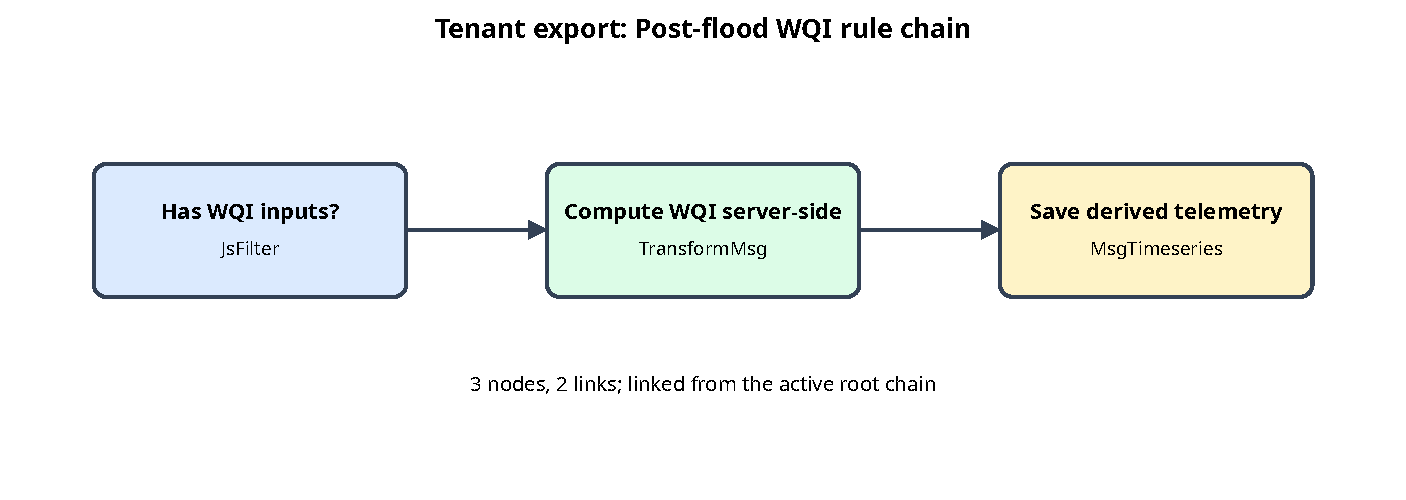
\includegraphics[width=\columnwidth]{figures/rule_chain.pdf}
\caption{Three-node server-side WQI chain reconstructed from the tenant export.}
\label{fig:rulechain}
\end{figure}

\begin{figure}[t]
\centering
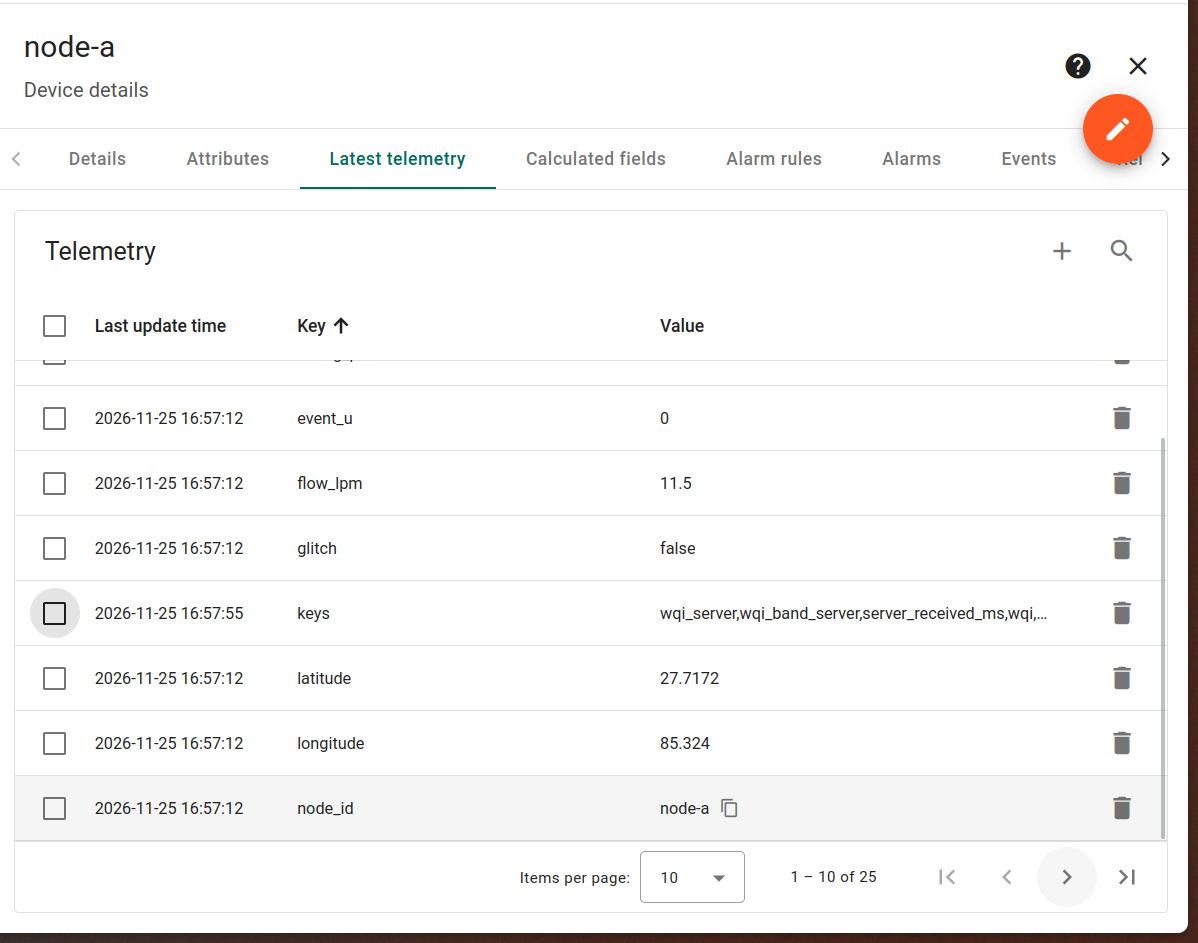
\includegraphics[width=\columnwidth]{figures/wqi_server_telemetry.png}
\caption{Latest Telemetry confirming \texttt{wqi\_server}, \texttt{wqi\_band\_server}
and \texttt{server\_received\_ms}.}
\label{fig:wqi}
\end{figure}

\begin{figure}[t]
\centering
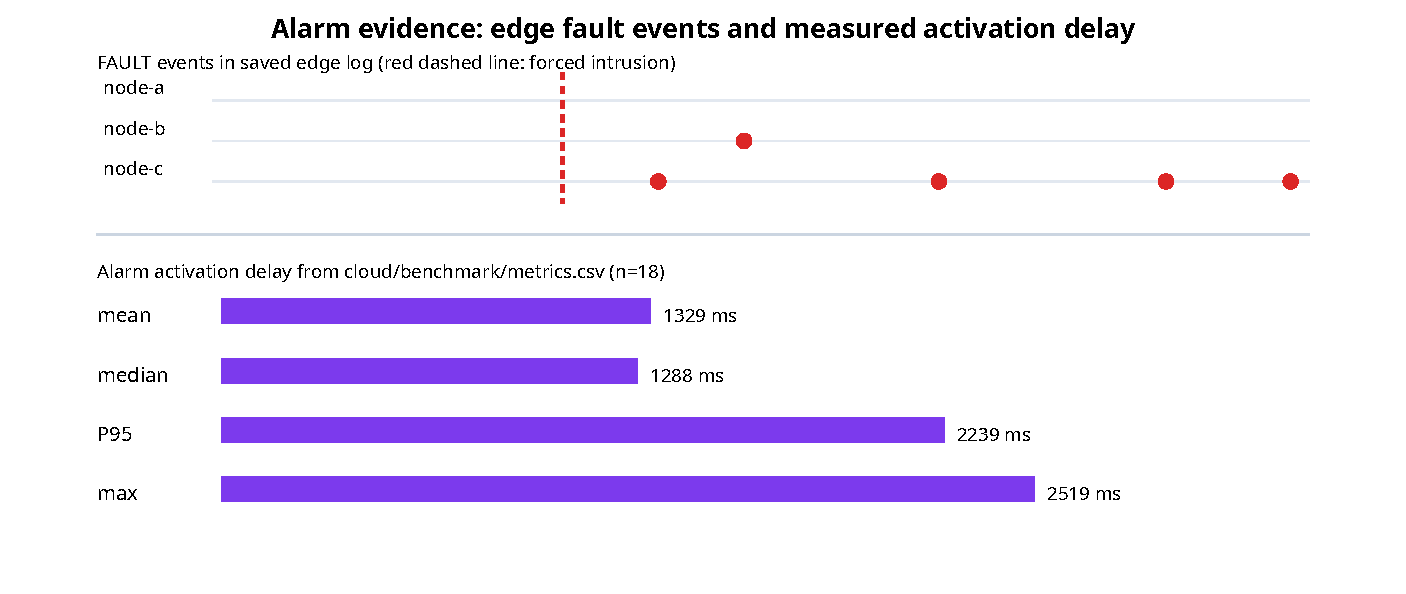
\includegraphics[width=\columnwidth]{figures/alarm_evidence.pdf}
\caption{Edge fault events from the saved log and the measured alarm-delay summary
from \texttt{cloud/benchmark/metrics.csv}; the tenant alarm-table screenshot was not
retained in the Cloud Track evidence set.}
\label{fig:alarms}
\end{figure}

\subsection{Benchmark Pipeline and Evidence Provenance}
\label{sec:benchmark-pipeline}

The benchmark is a separate Python module rather than a dashboard export, because
the six required metrics combine local queue state, parsed console events and
tenant REST state. In dry-run mode it reads only local files and reports
broker-dependent values as unavailable; with \texttt{--apply} it queries the
tenant using a JWT taken from the environment. The operator may restrict the
measurement window with \texttt{--start-ts} and \texttt{--end-ts}, select the
console log with \texttt{--log}, and choose the output stem with \texttt{--out};
these options produced the separate outage and no-outage reports. Raw telemetry
is queried with \texttt{agg=NONE} and a 50000-point limit, while alarm state is
read per device. Tokens and JWTs are never written to the JSON or CSV outputs.

\begin{table}[t]
\caption{Tenant API access details used by the benchmark}
\label{tab:endpoints}
\centering
\scriptsize
\begin{tabular}{@{}ll@{}}
\toprule
Access & Required behaviour \\
\midrule
Raw telemetry & \texttt{agg=NONE}; limit 50000 \\
Alarm history & per-device endpoint \\
Authentication & short-lived JWT from environment \\
Clock basis & epoch ms, NTP-synced hosts \\
\bottomrule
\end{tabular}
\end{table}

Credential handling is deliberately separated from measurement code. Device
access tokens and the tenant JWT are read from the local environment at run
time; \texttt{provision.py} substitutes the token placeholders only in memory,
and its dry-run mode performs no network calls. The submission builder rejects
secret-like strings before writing the archive, so a token copied into a note or
a test fixture cannot be submitted accidentally. Table~\ref{tab:secrets} lists
the classes of information that remain outside the repository.

\begin{table}[t]
\caption{Credential classes kept outside the repository}
\label{tab:secrets}
\centering
\scriptsize
\begin{tabular}{@{}ll@{}}
\toprule
Class & Handling \\
\midrule
Device access tokens & environment substitution at provisioning \\
Tenant JWT & short-lived, supplied per benchmark run \\
CA certificate & local path from environment \\
Submission archive & secret scanner before ZIP write \\
\bottomrule
\end{tabular}
\end{table}

Table~\ref{tab:evidence-files} maps each generated file to the evidence it
contains. Keeping the two raw reports alongside the consolidated report allows a
reviewer to recompute the table and to see why the outage latency is not used as
the live latency. The CSV is the canonical compact view: one row per metric with
the value, unit, sample count and provenance note.

\begin{table}[t]
\caption{Benchmark and evidence outputs}
\label{tab:evidence-files}
\centering
\scriptsize
\begin{tabular}{@{}ll@{}}
\toprule
File & Content \\
\midrule
\texttt{metrics.json} & consolidated six-metric report \\
\texttt{metrics.csv} & compact table with notes \\
\texttt{metrics\_outage.json} & raw 32~s outage run \\
\texttt{metrics\_live.json} & raw 177~s no-outage run \\
\texttt{latency\_scatter.svg} & latency against acquisition time \\
\texttt{edge\_*.log} & OUTAGE, REPLAY, PUBLISH, BUFFER events \\
\bottomrule
\end{tabular}
\end{table}

{\tiny
\begin{verbatim}
Algorithm 3  Six-metric benchmark pipeline
 1: rows <- local queue in [start_ts, end_ts]
 2: events <- parse OUTAGE/REPLAY/PUBLISH/BUFFER
 3: if apply: fetch telemetry, agg=NONE, limit=50000
 4: join tenant points by device id and original ts
 5: fetch alarms per device; pair with edge transitions
 6: compute latency, delivery and alarm-delay stats
 7: per outage: derive recovery and replay throughput
 8: count rows absent from tenant as data loss
 9: write JSON, CSV and optional latency plot
\end{verbatim}
}

\section{Tool Selection}
\label{sec:tools}

ThingsBoard was selected for device management, MQTT/TLS ingestion, per-device telemetry
with client timestamps, built-in alarm state machines, and dashboard export. SQLite at
the edge provides durable store-and-forward without a broker, and PUBACK confirmations
give an exact local sync count. The Python \texttt{paho-mqtt} client keeps the transport
swappable through a \texttt{NullPublisher} for dry runs.
Table~\ref{tab:tools} compares the selected stack with the two alternatives
considered against the assessment criteria. A raw MQTT broker with a custom web
dashboard is attractive for transport control, but device identity, credential
rotation, alarm latching, history retention and visualisation all have to be
implemented and verified separately. A Node-RED flow is convenient for rapid
correlation of simultaneous breaches, but it does not by itself provide a
device registry, per-device alarm state or an exportable dashboard; it is
therefore retained only as a future-work extension. ThingsBoard supplies those
platform services directly and, crucially, exposes its configuration as JSON
that can be committed as evidence. The cost is sensitivity to tenant-version
details, which Section~VIII-F documents.

\begin{table}[t]
\caption{Tool selection against assessment criteria}
\label{tab:tools}
\centering
\scriptsize
\begin{tabular}{@{}llll@{}}
\toprule
Criterion & Broker + UI & Node-RED & ThingsBoard \\
\midrule
Device identity & custom & custom & token \\
Alarm state & custom & nodes & native \\
History & custom DB & custom DB & built-in \\
Dashboard export & custom & custom & JSON \\
Correlation & custom & native & rule chain \\
Effort & high & medium & low \\
\bottomrule
\end{tabular}
\end{table}

\subsection{Validation and Test Coverage}

The repository contains 138 automated tests executed with \texttt{pytest}. They
are not performance benchmarks; they protect the state machines and artifact
generation that make the measured results reproducible. Table~\ref{tab:tests}
groups the test modules by the invariant they check. The ZIP builder tests also
reject secret-like strings, so a fresh tenant token or JWT cannot be committed
accidentally inside the submission archive.

\begin{table}[t]
\caption{Automated test coverage by invariant}
\label{tab:tests}
\centering
\scriptsize
\begin{tabular}{@{}ll@{}}
\toprule
Invariant & Test modules \\
\midrule
Sensor and DSP behaviour & \texttt{sensors}, \texttt{dsp}, \texttt{validity} \\
Alarm latching and severity & \texttt{hysteresis}, \texttt{runtime} \\
Buffer states and eviction & \texttt{storage}, \texttt{config} \\
MQTT chunking and identity & \texttt{publisher}, \texttt{runtime} \\
Scenario phase control & \texttt{scenarios} \\
Cloud artifacts and provisioning & \texttt{cloud\_provision}, \texttt{alarm\_rule\_imports} \\
Benchmark metric calculations & \texttt{cloud\_benchmark} \\
Submission archive hygiene & \texttt{build\_submission\_zip} \\
\bottomrule
\end{tabular}
\end{table}

\section{Results}

\subsection{Baseline, Intrusion, and Backfill}
\label{sec:baseline}

In the baseline phase the deterministic sensor model produces near-neutral pH,
low turbidity, moderate TDS and steady flow at all three nodes. Forcing the silt
intrusion raises turbidity with the configured amplitude and onset offset of each
node, while pH falls and TDS rises through the coupled model; the staged onsets
make the plume visible as a sequence across the fleet. The Cloud Track evidence
set contains saved console logs and benchmark reports rather than tenant
dashboard screenshots, so Figs.~\ref{fig:baseline} and~\ref{fig:alarms} are
generated from those records and are explicitly labelled as log-derived. The
multi-parameter chart retains the original acquisition timestamps after an
\texttt{o}/\texttt{o} outage cycle, so the backfill appears as a filled chronological
gap rather than a flat spike at recovery.

\begin{figure}[t]
\centering
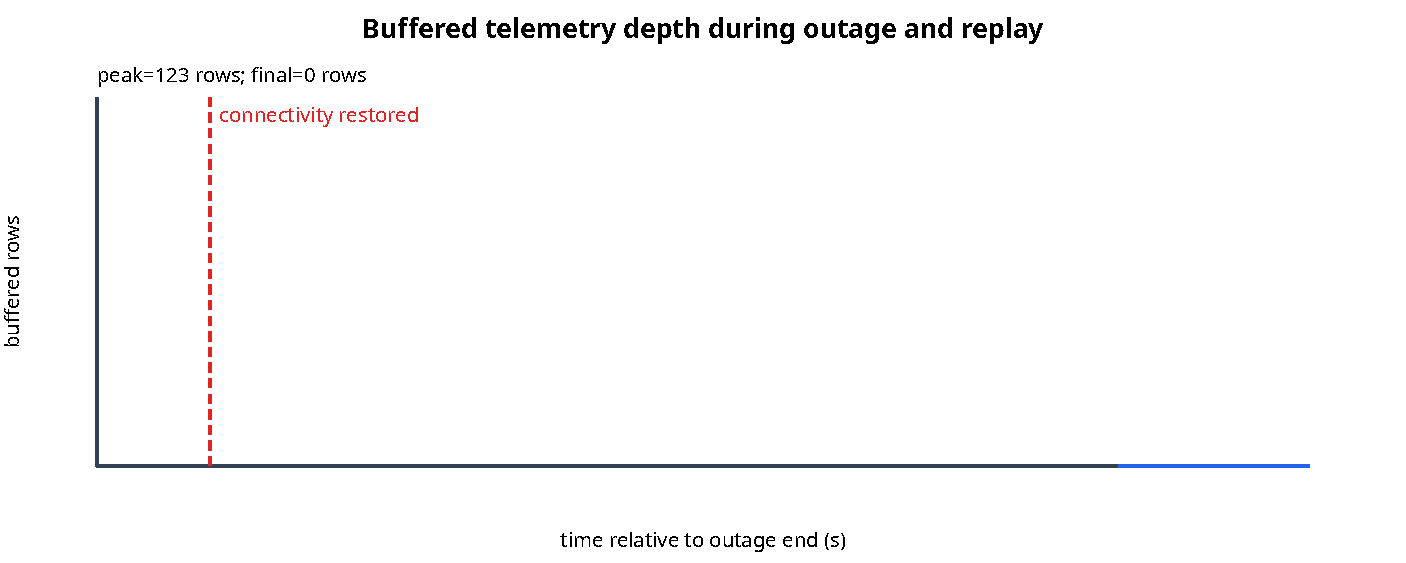
\includegraphics[width=\columnwidth]{figures/buffer_depth.pdf}
\caption{Buffered telemetry depth across the 32~s outage; replay restores the
original chronological sequence rather than creating a spike at recovery.}
\label{fig:backfill}
\end{figure}

Table~\ref{tab:scenario} gives the wall-clock log timestamps for the two saved
runs. The no-outage run is used for latency and alarm timing; the outage run is
used for delivery and replay. Keeping these timestamps in the manuscript allows
a reviewer to align the logs with the benchmark windows without re-running the
scenario controller.

\begin{table}[t]
\caption{Chronology of the two saved evidence runs}
\label{tab:scenario}
\centering
\scriptsize
\begin{tabular}{@{}ll@{}}
\toprule
Event & Log time (2026--11--25) \\
\midrule
Outage run start & 17:17:49.153 \\
Outage end & 17:18:21.157 \\
First zero buffer after replay & 17:19:23.100 \\
Clean run start & 17:29:50.368 \\
Forced silt intrusion & 17:30:50.231 \\
Clean run quit & 17:32:48.952 \\
\bottomrule
\end{tabular}
\end{table}

\subsection{Alerting Evidence}
\label{sec:alerting}

Under a forced silt intrusion, turbidity crossing 50~NTU raises High Turbidity
(Warning), crossing 200~NTU raises Gross Contamination (Critical), pH leaving the
6.5--8.5 interval raises pH Out of Range after three consecutive samples, and TDS above
500~ppm raises High TDS after the same debounce. A stuck-sensor injection raises Sensor
Fault, and a zero-flow interval raises Supply Interruption after 30~s. The tenant
alarm-table screenshot was not retained in this evidence set, so alarm evidence is
reported from the saved log and the REST alarm-creation times rather than from a UI
capture (Fig.~\ref{fig:alarms}). The activation delay is measured from the first
payload that breaches the threshold to the alarm creation time returned by the
ThingsBoard REST API. From
\texttt{cloud/benchmark/metrics.csv}, the measured mean alarm activation delay in the
no-outage live run was \textbf{1,329.2~ms over 18 alarm events} (median
1,288.5~ms, P95 2,239.3~ms), exceeding the ten-event minimum. In the outage run the
mean was 62,939.5~ms over 16 events, because alarms raised while rows were buffered
were only created after reconnection.

\begin{table}[t]
\caption{Alarm activation delay by measurement run}
\label{tab:alarm-runs}
\centering
\scriptsize
\begin{tabular}{@{}llll@{}}
\toprule
Run & Events & Mean & Interpretation \\
\midrule
Live & 18 & 1329.2~ms & connected threshold crossing \\
Outage & 16 & 62{,}939.5~ms & delayed until reconnect \\
\bottomrule
\end{tabular}
\end{table}

\subsection{Resilience and Buffer}
\label{sec:resilience}

The console log records \texttt{OUTAGE: START}, growing \texttt{BUFFER} totals, then
\texttt{OUTAGE: END}, \texttt{REPLAY} lines, and replayed \texttt{PUBLISH} lines carrying
the older epoch-millisecond timestamps. The \texttt{REPLAY} marker is preferred over
\texttt{PUBLISH} for throughput because \texttt{PUBLISH} also includes live samples
taken during the drain. Recovery is measured from connectivity restoration to the first
\texttt{BUFFER: total=0} line. From \texttt{cloud/benchmark/metrics.csv}: mean recovery
time \textbf{61.94~s} at a replayed buffer depth of \textbf{96~rows} (six 16-row
claims); mean flush throughput \textbf{1.55~rows/s}; message delivery ratio
\textbf{99.86\,\%}; and data loss \textbf{1 row (0.14\,\%)}. The 32~s outage and the
measurement window are stated in Section~\ref{sec:performance}.

\begin{figure}[t]
\centering
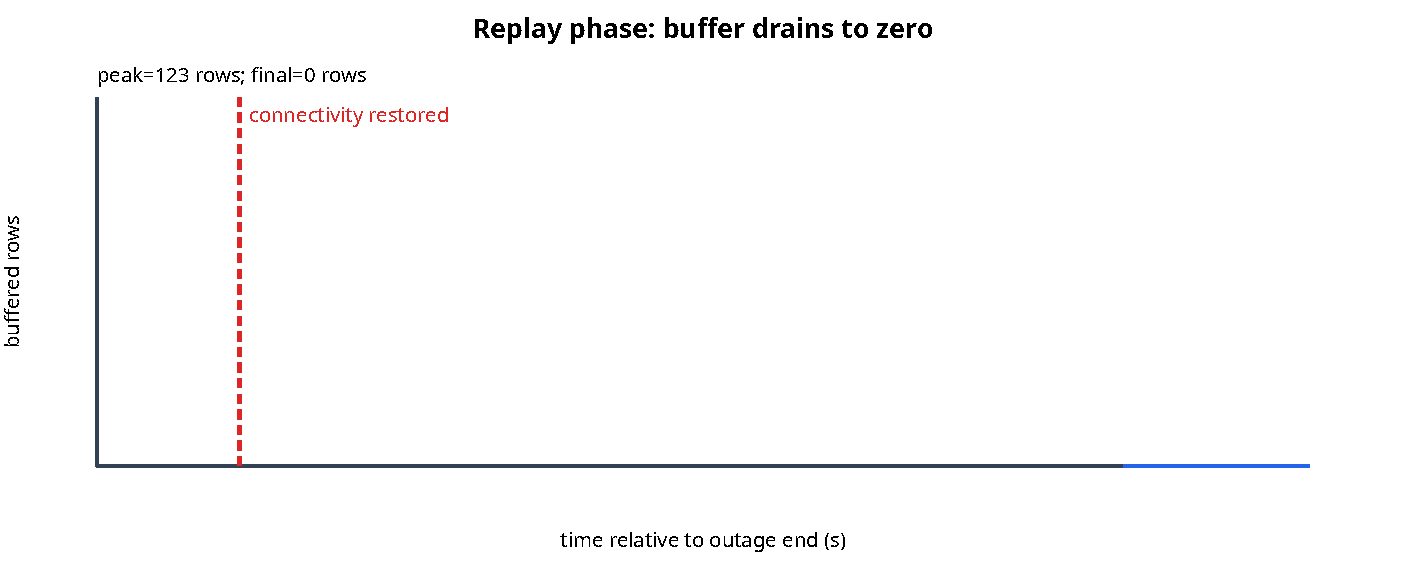
\includegraphics[width=\columnwidth]{figures/buffer_replay.pdf}
\caption{Buffer growth during outage and drain after reconnection.}
\label{fig:buffer}
\end{figure}

\subsection{Metric Definitions}
\label{sec:metric-defs}

Let $ts_i$ be the original acquisition timestamp of row $i$, $t^{\mathrm{srv}}_i$
the rule-chain value \texttt{server\_received\_ms}, $N_{\mathrm{gen}}$ the number of
locally generated rows, and $N_{\mathrm{tb}}$ the number of those rows whose
original timestamp appears in tenant telemetry. The latency and delivery
statistics are

\begin{equation}
L_i=t^{\mathrm{srv}}_i-ts_i,\qquad
D=100\,\frac{N_{\mathrm{tb}}}{N_{\mathrm{gen}}}.
\end{equation}

For alarm event $j$, the activation delay is
$A_j=t^{\mathrm{create}}_j-t^{\mathrm{edge}}_j$, where $t^{\mathrm{edge}}_j$ is the
first processed payload that qualifies for the rule and $t^{\mathrm{create}}_j$ is
the ThingsBoard alarm creation time. For a completed outage, let
$t_{\mathrm{end}}$ be the \texttt{OUTAGE: END} time, $t_0$ the first subsequent zero
buffer total, and $N_{\mathrm{replay}}$ the exact number of rows logged with the
\texttt{REPLAY} marker. Then

\begin{equation}
R=t_0-t_{\mathrm{end}},\qquad
Q=\frac{N_{\mathrm{replay}}}{R},\qquad
\ell=100\,\frac{N_{\mathrm{gen}}-N_{\mathrm{tb}}}{N_{\mathrm{gen}}}.
\end{equation}

Percentiles are computed on the values present in each report; where only one
outage was observed, the mean, median and P95 of recovery coincide and are
reported as a single sample rather than as a confidence interval.

\subsection{Performance Measurement}
\label{sec:performance}

Table~\ref{tab:metrics} collects the six mandatory metrics. Latency requires at least
200 messages with \texttt{server\_received\_ms} available from the linked water-quality
rule chain; the delivery ratio must be measured over a run that includes an outage; and
the alarm-delay figure requires at least ten alarm events. All values are copied from
\texttt{cloud/benchmark/metrics.csv} after a benchmark run against ThingsBoard with a
tenant JWT supplied through the environment. Two runs are reported. The outage run
spanned 09:38:40--11:33:18 UTC on 2026-11-25 in simulation time with a 32~s
connectivity outage, and provides the delivery ratio, throughput, recovery time
and data loss. Its latency sample ($n=709$, mean 270,767~ms) includes time spent in
the buffer, so it is a resilience bound rather than a live transfer time. The
no-outage run spanned 11:44:51--11:47:48 UTC with 530 generated and 528 confirmed
rows, and provides the representative live latency and alarm delay. The raw reports
are retained as \texttt{metrics\_outage.json} and \texttt{metrics\_live.json}.

\begin{table}[t]
\caption{Mandatory quantitative results}
\label{tab:metrics}
\centering
\tiny
\begin{tabular}{@{}lll@{}}
\toprule
Metric & Value & Basis \\
\midrule
Latency (mean/med/P95/max) & 1457.17/1444.00/2364.55/2939.00~ms & 528, live \\
Delivery ratio & 99.86\,\% & 707/708, outage \\
Alarm delay (mean) & 1329.22~ms & 18, live \\
Flush throughput & 1.55~rows/s & 96 replay rows \\
Recovery time & 61.94~s & depth 96 \\
Data loss & 1 (0.14\,\%) & outage \\
\bottomrule
\end{tabular}
\end{table}

Table~\ref{tab:runs} records which run supplies each metric. The separation is
necessary because an outage inflates latency without measuring network transfer
time: a row generated while disconnected may wait tens of seconds before it is
even eligible for publication. Delivery ratio, in contrast, is only meaningful
when a loss event occurred, so it is taken from the outage run.

\begin{table}[t]
\caption{Measurement run provenance}
\label{tab:runs}
\centering
\scriptsize
\begin{tabular}{@{}lll@{}}
\toprule
Run & Scope & Metrics used \\
\midrule
Outage, 32~s & 708 generated, 707 at tenant & delivery, throughput, recovery, loss \\
Live, 177~s & 530 generated, 528 confirmed & latency, alarm delay \\
\bottomrule
\end{tabular}
\end{table}

The host-only batch-size sweep times the complete enqueue, claim, publish, and
acknowledge path for 500 rows per size. The measured results in
\texttt{tools/batch\_results.csv} are reproduced in Table~\ref{tab:batch}.

\begin{table}[t]
\caption{Host-only batch-size sweep}
\label{tab:batch}
\centering
\small
\begin{tabular}{@{}rrr@{}}
\toprule
Batch size (rows) & Throughput (rows/s) & Elapsed (s) \\
\midrule
1 & 12992.94 & 0.038482 \\
10 & 22203.64 & 0.022519 \\
25 & 23001.16 & 0.021738 \\
50 & 23543.50 & 0.021237 \\
100 & 24330.85 & 0.020550 \\
200 & 23668.94 & 0.021125 \\
\bottomrule
\end{tabular}
\end{table}

\begin{figure}[t]
\centering
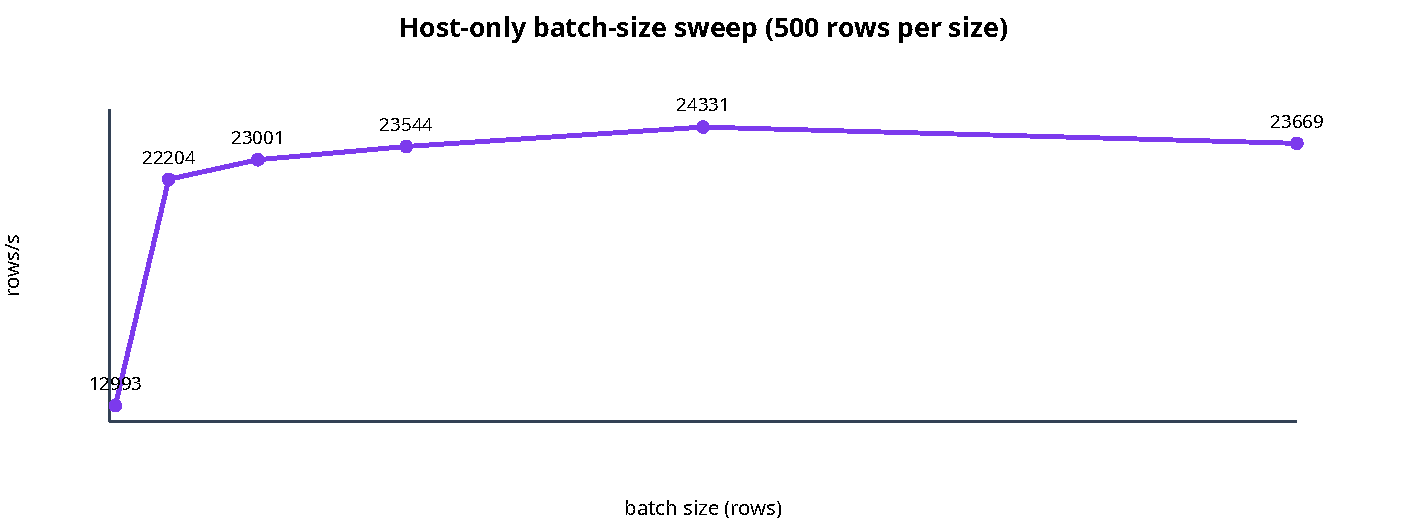
\includegraphics[width=\columnwidth]{figures/batch_sweep.pdf}
\caption{Measured host-only throughput against batch size; the peak is at 100 rows.}
\label{fig:batch}
\end{figure}

The highest host-only throughput was 24330.85~rows/s at a batch size of 100 rows, so
100 was used as the starting production value. The tenant, however, disconnects a
telemetry packet above roughly 2~KiB, so the publisher split each logical batch into
1800-byte MQTT chunks; the effective live batch is therefore smaller than the
host-only optimum. This distinction is important because the sweep is a local
storage-path result, not a broker measurement. Figure~\ref{fig:latency} shows the
latency scatter from the real-broker run.

\begin{figure}[t]
\centering
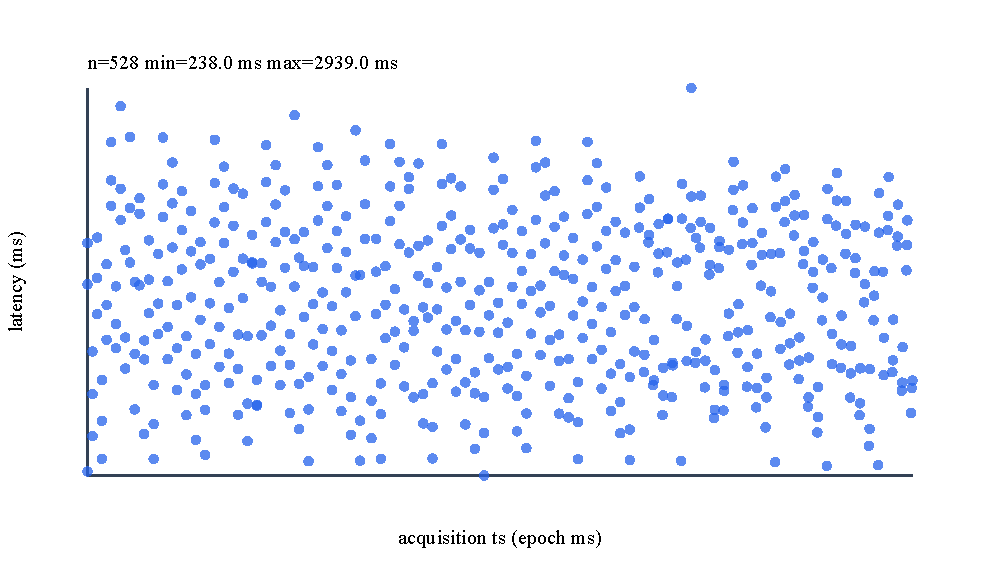
\includegraphics[width=\columnwidth]{figures/latency_scatter.pdf}
\caption{End-to-end latency against acquisition timestamp for the measured run.}
\label{fig:latency}
\end{figure}

\subsection{Latency Interpretation}
\label{sec:latency}

The live latency distribution is tightly centred: the median is 1444~ms and the
mean is 1457~ms over 528 samples, while P95 is 2365~ms and the maximum is
2939~ms. The small mean--median gap indicates that the reported latency is
dominated by the regular publish/acknowledge cycle rather than by rare stalls;
the tail is consistent with occasional multi-chunk flushes. These values are
computed from the tenant-side clock and the preserved acquisition timestamp, so
they include broker ingestion and rule-chain execution but not the sensor
sampling interval itself.

The outage report is deliberately excluded from this comparison. Its mean of
270~767~ms over 709 samples is larger because the same formula counts time spent
in the local buffer. Reporting that number as a network latency would conflate
resilience with transfer performance. The two-run design therefore answers two
different questions: how quickly a connected sample reaches the tenant, and how
much delay an interrupted sample accumulates before it is replayed.

\subsection{Measurement Methodology}

The benchmark reads the durable queue directly and parses the structured edge
log for \texttt{OUTAGE}, \texttt{REPLAY}, \texttt{PUBLISH} and
\texttt{BUFFER: total=0} events. With \texttt{--apply} it queries the tenant over
REST using a short-lived JWT provided through the environment; the token is
never written to a report or an exported artifact. Latency is computed as the
difference between the rule-chain value \texttt{server\_received\_ms} and the
original acquisition timestamp carried in each telemetry point. Delivery ratio
is the fraction of locally generated rows whose original timestamp appears in
the tenant's \texttt{ph} time series. Alarm delay pairs an edge
\texttt{active\_alarms} transition with the nearest subsequent ThingsBoard alarm
creation for the same device and alarm type. Recovery time is measured from
\texttt{OUTAGE: END} to the first zero buffer total, and flush throughput divides
the exact number of \texttt{REPLAY} rows by that interval.

The current tenant requires three API details that differ from older
documentation. Raw telemetry queries use \texttt{agg=NONE} in uppercase, because
lowercase is rejected with HTTP~400; the per-query limit is capped at 50000;
and alarm history is read per device from
\texttt{GET /api/alarm/DEVICE/\{uuid\}}, because the tenant-wide endpoints return
HTTP~405. Without these adaptations the benchmark silently reports N/A for
broker-dependent metrics. Two runs were measured: an outage run for resilience
metrics and a 177~s no-outage live run for latency and alarm delay. The tenant
JWT expired between them and was refreshed before the second query; both raw
reports are retained alongside the consolidated table.

\subsection{Operational Lessons and Limitations}

The live deployment exposed four tenant-specific behaviours that are relevant to
reproducibility. First, a telemetry MQTT packet above roughly 2~KiB caused an
immediate disconnect with return code~7 and no PUBACK; the publisher therefore
splits each logical batch into JSON arrays of at most 1800~bytes and requires an
acknowledgement for every chunk before the rows are marked synced. Second, three
publishers using an empty MQTT client id took over one another's sessions, so
each node now uses a stable identifier \texttt{post-flood-\{node\}}. Third, the
legacy alarm list embedded in an imported device profile was hidden in the
tenant UI, which is why the nine rules are additionally supplied as individual
importable alarm documents. Fourth, dashboard aliases were silently rejected,
so the eight widgets bind directly to the three verified device identifiers and
the map derives marker colour from raw telemetry when the \texttt{severity} key
is not stored.

Several limitations remain. The nodes are virtual, so no radio telemetry is
available and the requested \texttt{RSSI} widget is reported as N/A rather than
fabricated. Only one completed outage was measured, so throughput and recovery
statistics have a single sample and should be interpreted as a demonstration
rather than a confidence interval. The WQI uses surrogate indicators and is not
a substitute for microbiological testing. Finally, the latency measured during
the outage run includes time spent in the queue and is not a network transfer
time; this is why the no-outage run is used for the reported live latency.

Threats to validity are therefore specific rather than generic. Local timestamps
assume the edge host and tenant host remain NTP-synchronised; a clock offset
would bias latency and alarm delay by the same amount. The delivery ratio uses
the original acquisition timestamp as the join key, so a duplicated timestamp
from another node could be mismatched; the benchmark restricts the join to the
same device and telemetry key. The conclusions about tenant behaviour apply to
the tested Cloud release and may change after a platform upgrade. Finally, the
virtual sensor model reproduces the shape of a contamination event but cannot
validate field calibration of the surrogate WQI.

\section{Discussion}
\label{sec:discussion}

The evaluation can be read as four questions. First, does the edge preserve the
audit trail when the cloud disappears? The saved outage log shows that sampling
continued, the queue grew, replay used original timestamps, and the tenant
received 707 of 708 generated rows. The single missing row and the 61.94~s
recovery are reported rather than hidden; these numbers define the observed
envelope rather than an idealised guarantee.

Second, do the alarm rules report genuine excursions without flapping? The
implementation uses explicit deadbands and consecutive-sample counters, and the
live run produced 18 paired alarm events with a mean activation delay of
1329.2~ms. The outage run produced a much larger delay because the alarm could
not be created until the buffered payload reached the tenant. This contrast is
an important result: the edge decision is prompt, while tenant visibility
depends on connectivity.

Third, is the cloud configuration usable as a triage interface? The eight
widgets render from verified device identifiers, the WQI rule chain supplies
three server-side keys, and the profile assignment was confirmed on the tenant.
The map repair is a concrete example of evidence-driven configuration: latest
telemetry did not contain \texttt{severity}, so marker colour was derived from
fields that were actually present. An interface that merely imported without
error would not have passed this check.

Fourth, what limits the result? There was one completed outage, one tenant
release, and no radio telemetry from virtual nodes. The benchmark also depends
on clock synchronisation and on joining by acquisition timestamp. These limits
do not negate the measured result, but they bound its interpretation: the
prototype is a reproducible demonstration and a measurement pipeline, not a
validated production water-safety system.

\section{Assessment Deliverable Mapping}
\label{sec:deliverables}

Table~\ref{tab:deliverables} maps the submitted artifacts to the manuscript
sections that describe them. This is included so that a reviewer can move from a
rubric item to the corresponding evidence without searching the repository. The
mapping is deliberately artifact-first: each row names a file or directory that
is present in the submission archive, not an activity that was only performed in
the tenant UI.

\begin{table}[t]
\caption{Deliverables and their evidence locations}
\label{tab:deliverables}
\centering
\scriptsize
\begin{tabular}{@{}lll@{}}
\toprule
Deliverable & Section & Artifact \\
\midrule
Edge processing & II--IV & \texttt{edge/*.py} \\
Three devices and profile & VI-A & \texttt{cloud/artifacts/} \\
Eight-widget dashboard & VI-A & \texttt{dashboard\_triage.json} \\
Alarm rules and deadbands & VI-B & \texttt{alarm\_rules\_import/} \\
Server-side WQI & VI-B & \texttt{wqi\_rule\_chain.json} \\
Six-metric benchmark & VIII & \texttt{cloud/benchmark/} \\
Reproduction evidence & Appendix B & logs and exports \\
\bottomrule
\end{tabular}
\end{table}

The Cloud Track work described in Sections~VI-B, VIII-B--D, IX and X corresponds
to the individual allocation for Sambid Shrestha in Appendix~A of the group
submission. The edge sections are included because the benchmark and the alarm
evidence depend on their outputs; they are not reallocated here. This separation
keeps the measured values attributable to the component that produced them.

\section{Conclusion}
\label{sec:conclusion}

The prototype connects virtual water-quality sensors to ThingsBoard through an SQLite
store-and-forward buffer and MQTT over TLS. Original acquisition timestamps survive an
outage, and the cloud configuration exports a device profile, three devices, a
six-metric benchmark, a server-side water-quality rule chain, and an eight-widget triage
dashboard. Nine declarative alarm rules combine exact thresholds with deadbands and
consecutive-sample debounce, so excursions are reported without rapid flapping. The
completed demonstration produced a \textbf{1,329.2~ms} mean alarm activation delay over 18
live events, a \textbf{99.86\,\%} delivery ratio across the outage run,
\textbf{1.55~rows/s} flush throughput, and \textbf{1 row (0.14\,\%)} data loss. Within the
evaluated envelope, the chain satisfies the
sensing, resilience, visualisation, and quantitative-evaluation objectives of the task.
Table~\ref{tab:claims} maps each stated contribution to the evidence that
supports it, so that the conclusions can be checked without accepting the
architecture description on trust.

\begin{table}[t]
\caption{Contribution-to-evidence map}
\label{tab:claims}
\centering
\scriptsize
\begin{tabular}{@{}ll@{}}
\toprule
Contribution & Direct evidence \\
\midrule
Durable store-and-forward & outage log and replay metrics \\
Hysteresis alarm engine & nine imports and alarm-delay report \\
Server-side WQI & rule-chain export and telemetry capture \\
Eight-widget triage & dashboard JSON and artifact tests \\
Six-metric evaluation & consolidated benchmark CSV \\
\bottomrule
\end{tabular}
\end{table}

\section{Future Work}
\label{sec:future}

Critical alarms should trigger email or webhook notification so an operator is alerted
without watching the dashboard. A Node-RED flow could correlate simultaneous breaches
across \texttt{node-a}, \texttt{node-b}, and \texttt{node-c} to localise the contaminated
segment of the distribution network. The accelerated demonstration constants should be
replaced by production time constants of 1800~s for sustained zero flow and 600~s for
the derivative window. A real sensing node would also provide radio telemetry, allowing
the requested \texttt{RSSI} widget to be populated instead of marked N/A; the
surrogate-indicator calibration would need field validation before the index is used
operationally.

The immediate next step is a longer field trial with real sensors and at least
five completed outages, so that recovery and throughput can be reported with a
variance instead of a single observation. The tenant-side alarm rules should then
be re-measured against the edge latch to confirm that the copied thresholds and
deadbands produce the same active set after a deadband crossing. Finally, the
batch size should be re-tuned against the live broker: the host-only optimum of
100~rows/s does not account for the 1800-byte packet ceiling or PUBACK latency,
and the current live configuration therefore trades peak local throughput for
deterministic acknowledgement.

\appendices{}

\section{Telemetry Payload Contract}
\label{app:payload}

Each buffered row is a JSON object with an acquisition timestamp in epoch
milliseconds and a flat \texttt{values} map. Table~\ref{tab:payload} lists the
published keys. The tenant also derives \texttt{wqi\_server},
\texttt{wqi\_band\_server} and \texttt{server\_received\_ms} from the linked rule
chain; those keys are stored separately so that the edge-computed
\texttt{wqi} and \texttt{wqi\_band} remain authoritative.

\begin{table}[t]
\caption{Telemetry payload keys}
\label{tab:payload}
\centering
\scriptsize
\begin{tabular}{@{}lll@{}}
\toprule
Key & Type / unit & Origin \\
\midrule
\texttt{node\_id} & string & identity \\
\texttt{ts} & epoch ms & acquisition \\
\texttt{latitude}, \texttt{longitude} & degrees & location \\
\texttt{ph}, \texttt{ph\_25} & pH / compensated & sensor / DSP \\
\texttt{turbidity\_ntu} & NTU & sensor \\
\texttt{tds\_ppm} & ppm compensated & sensor / DSP \\
\texttt{water\_temp\_c} & $^\circ$C & sensor \\
\texttt{flow\_lpm} & L/min & sensor \\
\texttt{wqi}, \texttt{wqi\_band} & index / string & edge WQI \\
\texttt{severity} & string & alarm severity \\
\texttt{active\_alarms} & CSV string & alarm names \\
\texttt{buffer\_depth} & integer & queue depth \\
\texttt{node\_inactive} & boolean & 90~s alarm \\
\texttt{validity\_flags} & CSV string & gate diagnostics \\
\texttt{sensor\_fault} & boolean & fault flag \\
\bottomrule
\end{tabular}
\end{table}

\section{Reproduction and Evidence Inventory}
\label{app:repro}

The complete chain can be reproduced from the repository without credentials:
the dry-run publisher uses a \texttt{NullPublisher} and the benchmark reports
broker-dependent metrics as unavailable. A live reproduction needs a local,
gitignored \texttt{.env} containing the three device access tokens, the tenant
host and a short-lived tenant JWT. The commands used for the measurements in
this paper were:

{\tiny
\begin{verbatim}
python -m edge.cli --mqtt --tick-seconds 1
python -m cloud.benchmark --apply --plot
python -m cloud.benchmark --apply --plot \
    --start-ts 1795607091933 --end-ts 1795607268807 \
    --log evidence/edge_clean_final.log --out cloud/benchmark/live
python tools/build_paper_figures.py
rsvg-convert -f pdf -o paper/figures/latency_scatter.pdf \
    cloud/benchmark/latency_scatter.svg
python tools/build_submission_zip.py --group <GROUP>
\end{verbatim}
}

A minimum review checklist follows the same order: (i) inspect the two saved
logs for the phase and outage markers in Table~\ref{tab:scenario}; (ii) open the
consolidated CSV and confirm that the sample counts meet the task minima;
(iii) compare the two raw JSON reports with the provenance table; (iv) confirm
that the WQI rule-chain export is linked from the root chain and that Latest
Telemetry contains the three derived keys; and (v) build the archive and verify
that no credential-like strings appear in it. This sequence checks the evidence
chain from acquisition to submission without requiring access to the tenant
during review.

The evidence bundle is indexed in Table~\ref{tab:inventory}. The automated test
suite covers alarm-import generation, dashboard construction, secret rejection
in the ZIP builder, publisher chunking and client identity, and the benchmark
metric calculations; all tests pass at submission time.

\begin{table}[t]
\caption{Submitted evidence inventory}
\label{tab:inventory}
\centering
\scriptsize
\begin{tabular}{@{}ll@{}}
\toprule
Group & Files \\
\midrule
Tenant exports & profile PNG; root/WQI chain JSON \\
Runtime evidence & outage/clean logs; telemetry PNG \\
Benchmark outputs & metrics JSON/CSV; raw reports \\
Cloud artifacts & dashboard JSON; nine alarm imports \\
Generated figures & SVG/PDF in \texttt{paper/figures} \\
\bottomrule
\end{tabular}
\end{table}

The nine alarm-rule import files are listed in
Table~\ref{tab:alarm-files}. Six implement the mandatory direct thresholds; the
remaining three mirror edge-derived conditions that the tenant can evaluate
from published fields without a custom alarm chain.

\begin{table}[t]
\caption{Alarm import documents}
\label{tab:alarm-files}
\centering
\scriptsize
\begin{tabular}{@{}ll@{}}
\toprule
Rule & Import document \\
\midrule
High Turbidity & \texttt{high\_turbidity.json} \\
Gross Contamination & \texttt{gross\_contamination.json} \\
pH Out of Range & \texttt{ph\_out\_of\_range.json} \\
High TDS & \texttt{high\_tds.json} \\
Supply Interruption & \texttt{supply\_interruption.json} \\
Node Inactive & \texttt{node\_inactive.json} \\
Rapid Turbidity Rise & \texttt{rapid\_turbidity\_rise.json} \\
Severe pH Persistence & \texttt{severe\_ph\_persistence.json} \\
Sensor Fault & \texttt{sensor\_fault.json} \\
\bottomrule
\end{tabular}
\end{table}

\section{Verified Tenant Artifacts}
\label{app:tenant}

Table~\ref{tab:tenant} records what was checked on the tenant rather than only
in the repository. The distinction matters because a JSON file can be valid yet
remain unassigned, unlinked, or hidden by a tenant UI after import. Each row
therefore pairs a configuration artifact with the observed tenant state and the
saved evidence file.

\begin{table}[t]
\caption{Tenant-side verification of committed artifacts}
\label{tab:tenant}
\centering
\scriptsize
\begin{tabular}{@{}lll@{}}
\toprule
Artifact & Verified state & Evidence \\
\midrule
Device profile & three devices assigned & assignment PNG \\
Root chain & export saved & root-chain JSON \\
WQI chain & linked; derived keys present & chain JSON + PNG \\
Dashboard & eight widgets bound & dashboard JSON \\
Alarm rules & nine imports available & import directory \\
\bottomrule
\end{tabular}
\end{table}

\section{Schematic Telemetry Payload}
\label{app:payload-schema}

Listing~1 shows the payload shape used by the publisher. The angle-bracket
terms are type placeholders, not captured values; the purpose is to document the
contract that both the dashboard and the benchmark rely on. Every row carries
its acquisition timestamp outside the \texttt{values} map, which is what allows
replayed records to retain their original chronological position.

{\tiny
\begin{verbatim}
Listing 1: Schema of one buffered telemetry row
{
  "ts": <epoch_ms>,
  "values": {
    "node_id": "<node-id>",
    "latitude": <deg>, "longitude": <deg>,
    "ph": <ph>, "ph_25": <ph>,
    "turbidity_ntu": <ntu>,
    "tds_ppm": <ppm>,
    "water_temp_c": <c>, "flow_lpm": <lpm>,
    "wqi": <index>, "wqi_band": <str>,
    "severity": <str>, "active_alarms": <csv>,
    "buffer_depth": <rows>,
    "node_inactive": <bool>,
    "validity_flags": <csv>,
    "sensor_fault": <bool>
  }
}
\end{verbatim}
}

\bibliographystyle{IEEEtran}
\bibliography{references}

\end{document}
